\subsection{Reflecting Boundaries}

\begin{frame}
	\frametitle{4) Periodic Boundaries with Vision}
	\textbf{Implementation.}
	\begin{itemize}
	    \item Just particles in circle segment defined by vision angle $\varphi$ are considered
	\end{itemize}
	\begin{figure}[H]
  		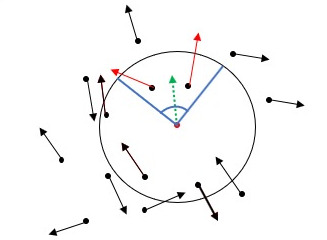
\includegraphics[width=0.4\textwidth]{images/chapter4/particle_vision.jpeg} 
	\end{figure}
\end{frame}

\begin{frame}
	\frametitle{4) Periodic Boundaries with Vision}
	\textbf{Trajectory.} Comparing Angles.
	\begin{itemize}
	    \item $\rho = 400, v = 0.03, R = 0.03, D_{\text{rot}} = 0.01, \Delta t = 1.0$
	    \item $v_a$ grows with vision angle
	\end{itemize}
	\begin{figure}[H]
  		\includegraphics[width=\textwidth]{images/chapter4/trajectory_comp_N_20_L_1.000000_v_0.030000_R_0.030000_D_0.010000.png} 
  		%\caption*{Cantillano C., Grundpraktikum 2: Halbleiterbauelemente. Internal Proceedings. University of Innsbruck , 2021.}
	\end{figure}
\end{frame}

\begin{frame}
	\frametitle{4) Periodic Boundaries with Vision}
	\textbf{Configurations.} Comparing Angles.
	\begin{itemize}
	    \item $\rho = 400, v = 0.03, R = 0.03, D_{\text{rot}} = 0.01, \Delta t = 1.0$
	    \item Flock size grows with vision angle
	\end{itemize}
	\begin{figure}[H]
  		\includegraphics[width=\textwidth]{images/chapter4/configuration_comp_N_20_L_1.000000_v_0.030000_R_0.030000_D_0.010000.png} 
  		%\caption*{Cantillano C., Grundpraktikum 2: Halbleiterbauelemente. Internal Proceedings. University of Innsbruck , 2021.}
	\end{figure}
\end{frame}

\begin{frame}
	\frametitle{4) Periodic Boundaries with Vision}
	\textbf{Phase transitions.} 2D Levels in parameter space.
	\begin{itemize}
	    \item $R$ against $\sqrt{2D_{\text{rot}}\Delta t}$
	    \item Region of ordered phase increases with vision angle
	\end{itemize}
	\begin{figure}[H]
  		
\includegraphics[width=0.9\textwidth]{images/chapter4/phase_comp_N_20_L_1.000000_v_0.030000_R_0.030000_D_0.010000.png} 
  		%\caption*{Cantillano C., Grundpraktikum 2: Halbleiterbauelemente. Internal Proceedings. University of Innsbruck , 2021.}
	\end{figure}
\end{frame}



